\documentclass[a4paper,11pt]{report}
\usepackage[utf8]{inputenc}
\usepackage[T1]{fontenc}
% Mes polices: times, newcent, default
\usepackage{times} % probleme d'accent avec charter
\usepackage[francais]{babel}
\usepackage[top=3cm, bottom=3cm, left=3cm, right=3cm]{geometry}
\usepackage{array}
\usepackage{fancyhdr}
\usepackage{textcomp}
\usepackage{graphicx}
\usepackage{hyperref}
\setcounter{secnumdepth}{3}

\makeatletter
\def\clap#1{\hbox to 0pt{\hss #1\hss}}%
\def\ligne#1{%
\hbox to \hsize{%
\vbox{\centering #1}}}%
\def\haut#1#2#3{%
\hbox to \hsize{%
\rlap{\vtop{\centering #1}}%
\hss
\clap{\vtop{\centering #2}}%
\hss
\llap{\vtop{\centering #3}}}}%
\def\bas#1#2#3{%
\hbox to \hsize{%
\rlap{\vbox{\centering #1}}%
\hss
\clap{\vbox{\centering #2}}%
\hss
\llap{\vbox{\centering #3}}}}%
\def\maketitle{%
\thispagestyle{empty}\vbox to \vsize{%
\haut{}{\@blurb}{}
\vfill
\vspace{1cm}
\begin{flushleft}
\usefont{OT1}{ptm}{m}{n}
\huge \@title
\end{flushleft}
\par
\hrule height 4pt
\par
\begin{flushright}
\usefont{OT1}{phv}{m}{n}
\Large \@author
\par
\end{flushright}
\vspace{1cm}
\vfill
\vfill
%\bas{}{\@location, le \@date}{}
\bas{}{\@date}{}
}%
\cleardoublepage
}
\def\date#1{\def\@date{#1}}
\def\author#1{\def\@author{#1}}
\def\title#1{\def\@title{#1}}
\def\location#1{\def\@location{#1}}
\def\blurb#1{\def\@blurb{#1}}
\date{Année académique 2014 – 2015}
\location{Bruxelles}
\makeatother
\title{ \textsc{CityLord} :
\textsc{Software Requirements Document}\\}

\author{\textsc{\textbf{Groupe 2}}\newline Zakaria \textsc{Aharrar} – Hakim \textsc{Boulahya} – David \textsc{Fishel} – Cédric \textsc{Orinx} – Gabriel \textsc{Ortega} – Kaio \textsc{Lopes}}
\location{Bruxelles}
\blurb{%
UNIVERSITÉ LIBRE DE BRUXELLES\\
Faculté des sciences\\
\textsc{\textbf{Département d'informatique}}
%\textbf{Rapport de stage en entreprise}\\
\\[2em]
Enseignants : 
Joël GOOSSENS, Christian HERNALSTEEN\\
Cours : INFO-F-209 – Projet d'année 2
}%


\begin{document}
%\fancypagestyle{empty}{
%  \fancyhf{}
%  \fancyhead[L]{
\includegraphics[scale=1]{logoulb.jpg}}
%}
\maketitle
\tableofcontents
\clearpage

\chapter{Introduction}
\section{But du projet}
\paragraph{}
Nous allons implémenter CityLord, un jeu de gestion de ville multi-joueur.
Celui-ci se jouera entre 2 à 8 joueurs différents qui pourront acheter, vendre, ou améliorer des bâtiments, dans une même villes.
Le but du jeu est le même pour chaque joueur, être le dernier propriétaire dans la ville, ou bien être celui avec le plus grand capital (argent+valeur des bâtiments) à la fin du temps imparti.

Au départ, chaque joueur commence avec une parcelle prise au hasard, et une somme modeste lui permettant d'acheter un nombre limité de propriété (1 voir 2 parcelles ou bâtiments).

Pour gagner de l'argent, des visiteurs (non-controlé par les joueurs) doivent entrer dans un de leur établissement, y rester une durée déterminée, leur donner l'argent adapté à l'établissement où il se trouve, et disparaitra ensuite de la partie.
Un visiteur ne peut apparaitre qu'à des endroits prédéfini sur la carte (ex: station de métro), il suivra alors un chemin également prédéfini (ex: vers la sortie de la ville), et entrera dans un établissement qu'il croise, si celui-ci l'interesse.
Ce sera donc aux joueurs de bien positionner leurs bâtiments là où ils ont le plus de chances d'attirer un grand nombre de visiteur.

Les bâtiments ne peuvent accueuillir qu'un nombre limité de visiteur en même temps, accepter une même somme par visiteur, et se débarasser d'un visiteur qu'après une certaine durée.
Un joueur peut, s'il le souhaite et pour un certain coût, amélioré son bâtiment, et alors augmenter la capacité maximale, la recette par visiteur et diminuer la durée d'occupation d'un visiteur.

Si un joueur est en faillite, à cause d'un coût d'entretien trop élévé face aux recettes, il sera alors obligé de vendre des propriétés. Il mettra alors sa propriété (parcelle+bâtiment) dans le catalogue de vente, ouvert à tous les joueurs.
Il peut également s'il le souhaite, supprimer son bâtiment, ce qui réduira grandement les coût d'entretien, mais rendera les recettes nulles. (Une parcelle vide à un coût d'entretien, mais pas de revenu, ceci est pour éviter qu'un joeur achète tous les emplacements simplement pour empêcher les autres de construire).

\newpage
\section{Glossaire}
\begin{itemize}
 \item \textbf{Système:} Un système est un ensemble d'éléments interagissant entre eux selon certains principes ou règles. Dans ce cas, il s’agit du programme.
 \item \textbf{Point-and-click:} se dit d’une des actions qu'un utilisateur peut effectuer sur une interface utilisateur graphique avec pointeur.
L'utilisateur déplace le pointeur avec un dispositif de pointage (souris, manette de jeu) sur un emplacement particulier de l'écran d'ordinateur,
puis il appuie sur un bouton du dispositif pour déclencher l'action .
 \item \textbf{Serveur:} Un serveur est ordinateur dédié à l'administration d'un réseau informatique. Il gère l'accès aux ressources et aux périphériques et les connexions des différents utilisateurs.
 \item \textbf{Réseau informatique:}Ensemble des moyens matériels et logiciels mis en œuvre pour assurer les communications entre ordinateurs.
 \item \textbf{Pseudo:}Un pseudonyme est un nom d'emprunt qu'une personne porte pour exercer une activité sous un autre nom que celui de son identité officielle.
 \item \textbf{Map:}Carte prédéfinie, représentant une ville.
 \item \textbf{Catalogue:}Liste reprenant toutes les propriétés mises en vente par les joueurs ou par la villes.
\end{itemize}

\newpage
\section{Historique du document}
\begin{description}
	\item[1.9] (06/02/15) : Modification du But du projet, ajout au glossaire \& index +précondition "Construire"  - David
	\item[1.8] (15/12/14) : Mise à jour des exigences de domaine - Cédric
    \item[1.7] (14/12/14) : Ajout des déscriptions textuelles des uses cases (Premiers achats,Construire-Améliorer-Détruire,Achats entre joueurs) - David
    \item[1.6] (12/12/14) : Rajout et correction des déscriptions textuelles des use case, et ajout des exigences de domaine - Hakim
    \item[1.5] (11/12/14) : Déscriptions textuelles de l'interface de connexion - Kaio
    \item[1.4] (11/12/14) : Exigences fonctionnelles (Besoins de l'utilisateur) et ajout dans le glossaire et l'index de termes - David
    \item[1.3] (11/02/14) : Ajout du diagramme de classe - Equipe
    \item[1.2] (10/02/14) : Ajout des premières \textit{use case} - Zakaria
    \item[1.1] (10/02/14) : Première version. (Aharrar Zakaria) Contient les points 1.1, 1.2, 1.3, 2 et 2.1 (partiellement) - Zakaria
    \item[1.0] (09/12/14) : Création du document - Hakim
    
\end{description}


\newpage
\chapter{Besoins de l'utilisateur}
\section{Exigences fonctionnelles}
\subsection{Interface de connexion}
\begin{figure}[ht]
    \makebox[\linewidth]{
        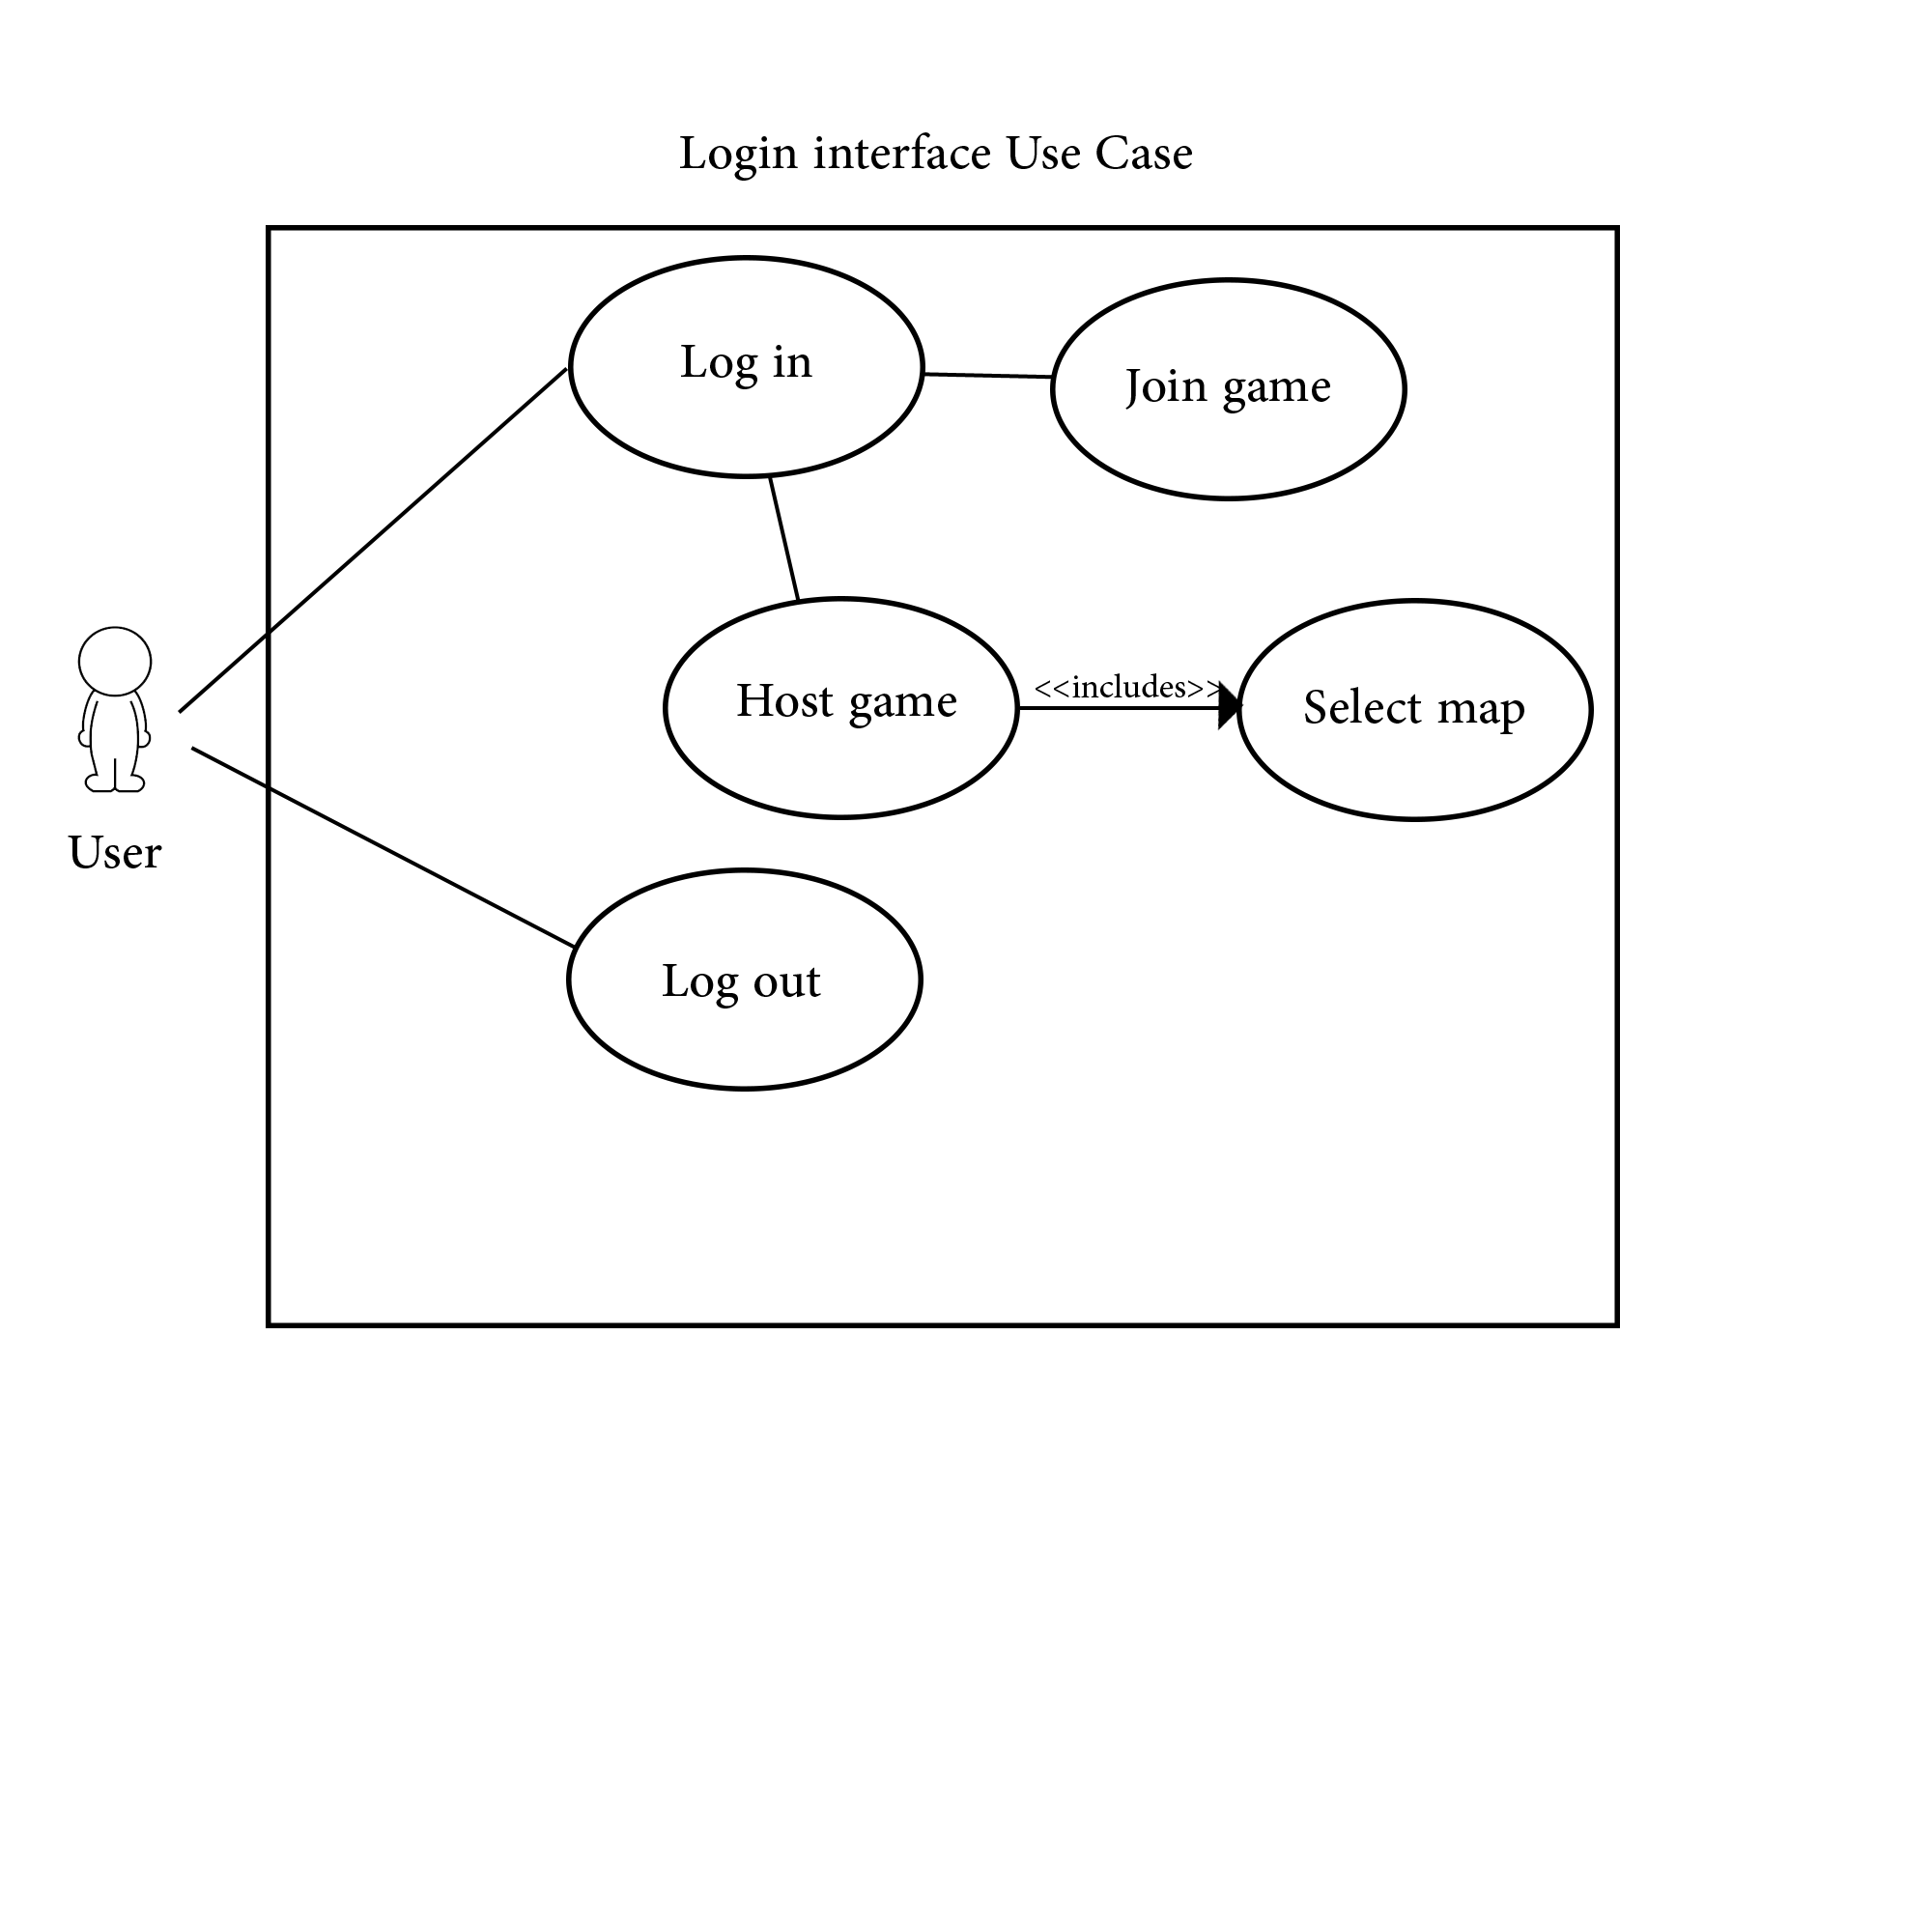
\includegraphics[width=550pt]{uml/useCaseDiagrams/loginUseCase.png}
    }
    \caption{Use Case Login/Logout}
\end{figure}
\subsubsection{Log in}
\paragraph{Préconditions}
\begin{itemize}
 \item Le jeu doit être ouvert.
 \item L'utilisateur ne doit pas être connecté.
\end{itemize}
\paragraph{Postconditions}
\begin{itemize}
 \item L'utilisateur est connecté.
\end{itemize}
\paragraph{Cas général}
Une fois le jeu démarrer, l'utilisateur peut se connecté insérant un nom d'utilisateur existant et le mot de passe associé
[Exception : mauvais mot de passe ou pseudo non-existant].
Une fois toutes les informations entré, l'utilisateur appuie sur le bouton \og \textit{Connect} \fg, et l'utilisateur est
connecté. Un utilisateur non-enregistré peut également créer un nouveau pseudo unique
et lui associé mot de passe en appuyant sur le bouton \og \textit{Create} \fg
[Exception: pseudo déjà utilisé].
Une fenêtre va ensuite s'ouvrir et lui demandé d'entrer les informations nécessaires 
[Exception: aucun pseudo et/ou mot de passe entré]. Ceci ajoutera sur le serveur un nouvel utilisateur avec comme
pseudo et mot de passe associés ceux entrés dans les zones appropriées, et connectera l'utilisateur automatiquement.
\paragraph{Exceptions}
\begin{itemize}
 \item \textit{Mauvais mot de passe ou pseudo non-existant:} Après la pression du bouton \og \textit{Connect} \fg
 ,sur la même vue, une remarque apparait, en une couleur fortement
 perceptible, et indique à l'utilisateur que les informations entrées sont incorrectes. La fenêtre de connexion reste ouverte et
 demande à l'utilisateur de réentrer son pseudo et son mot de passe.
 \item \textit{Pseudo déja utilisé:} Après la pression du bouton \og \textit{Create} \fg,
 sur la même vue, une remarque apparait, en une couleur fortement
 perceptible, et indique à l'utilisateur que le pseudo demandé est déjà utilisé. La fenêtre de création reste ouverte
 et demande à l'utilisateur de réentrer un nouveau pseudo.
 \item \textit{Aucun pseudo et/ou mot de passe entré:} Dans les deux cas - de connexion ou de création - si l'utilisateur
 manque d'entrer une information, après du bonton associé à la fenêtre en premier plan, sur la même vue,
 une remarque apparait, en une couleur fortement perceptible, et indique à l'utilisateur l'information manquante. La
 fenêtre reste ouvert et demande à l'utilisateur d'entrer cette information pour continuer la connexion ou la création.
\end{itemize}

\subsubsection{Log out}
\paragraph{Préconditions}
\begin{itemize}
 \item L'utilisateur doit être connecté.
\end{itemize}
\paragraph{Postconditions}
\begin{itemize}
 \item L'utilisateur est déconnecté.
 \item La fenêtre du jeu est fermé.
\end{itemize}
\paragraph{Cas général}
Un joueur peut se déconnecté à n'importe quel moment. Si il est en partie, il la quitte automatiquement. L'utilisateur
est ensuite déconnecté et la fenêtre du jeu se ferme.
\paragraph{Excéptions} Néant.
\subsubsection{Join game}
\paragraph{Préconditions}
\begin{itemize}
 \item L'utilisateur est connecté.
\end{itemize}
\paragraph{Postconditions}
\begin{itemize}
 \item L'utilisateur est dans une partie.
\end{itemize}
\paragraph{Cas général}
Un utilisateur client peut rejoindre une partie en appuyant sur le bouton \og \textit{Join Game} \fg 
du menu principal.
Il est ensuite envoyé dans l'écran de séléction du jeu, ou il lui est possible de voir toutes les parties lancées sur le
même serveur et visualiser les différentes informations sur chacunes d'elles, comme le temps passé depuis le lancement
de la partie ou le status de celle-ci.
[Exception: la partie est complète]
Après avoir rejoins une partie, si celle-ci n'est pas commencé le joueur est placé dans l'acceuil où il peut
voir tous les joueurs en attente - du début de la partie -, dont l'hote de la partie, et la carte choisie. Il lui
est également possible de chatter avec les autres joueurs. 
[Exception: Hôte ferme la partie]
Dans le cas où la partie est déjà comencé le joueur reçoit de l'argent.
\paragraph{Exceptions}
\begin{itemize}
 \item \textit{La partie est complète:} Une fenètre s'ouvre indiquant a l'utilisateur que la partie est complète
 et donc injoingnable. Une fois cette fenêtre fermée l'utilisateur est ramené au menu de selection.
 \item \textit{Hôte ferme la partie:} L'utilisateur client est ramené au menu de selection [pour plus d'informations, voir
 Host Game]. 
\end{itemize}

\subsubsection{Host game}
\paragraph{Obligations spéciales}
\begin{itemize}
 \item Inclut Select Map.
\end{itemize}
\paragraph{Préconditions}
\begin{itemize}
 \item L'utilisateur doit être connecté.
\end{itemize}
\paragraph{Postconditions}
\begin{itemize}
 \item L'utilisateur hôte et les utilisateurs clients sont dans une partie.
\end{itemize}
\paragraph{Cas général}
L'utilisateur hôte est capable de créer une partie en appuyant sur le bouton \og \textit{Host game} \fg du menu principal.
Une fois créée, l'hôte peut choisir une carte. L'hôte peut également chatter avec les autres utilisateurs.
L'hôte peut également afermer l'acceuil en appuyer sur le bouton \og \textit{Close lobby} \fg. Tous les clients
présent dans l'acceuil est renvoyé à l'écran de selection, tandis que l'hôte est renvoyé dans le menu principal.
Quand il y a assez de joueur - minimum 2 et maximum 8 hôte inclut - le bouton \og \textit{Start game} \fg s'active.
Quand il est cliqué, chaque utilisateur présent dans l'acceuil est lancé dans la partie et reçoit de l'argent.
\paragraph{Exceptions} Néant.

\newpage
\subsubsection{Select map}
\paragraph{Obligations spéciales}
\begin{itemize}
 \item Est inclut dans Host Game
\end{itemize}
\paragraph{Préconditions}
\begin{itemize}
 \item L'hôte doit être dans un acceuil.
\end{itemize}
\paragraph{Postconditions}
\begin{itemize}
 \item La carte choisie est chargée.
\end{itemize}
\paragraph{Cas général}
L'utilisateur hôte peut choisir une carte dans une liste prédéfinie de carte. Quand tous les éléments pour démarrer la partie
sont réunis [pour plus d'informations, voir Host Game], la carte est chargée.
\paragraph{Exceptions} Néant.

\newpage
\subsection{Achats libres}
\begin{figure}[ht]
    \makebox[\linewidth]{
        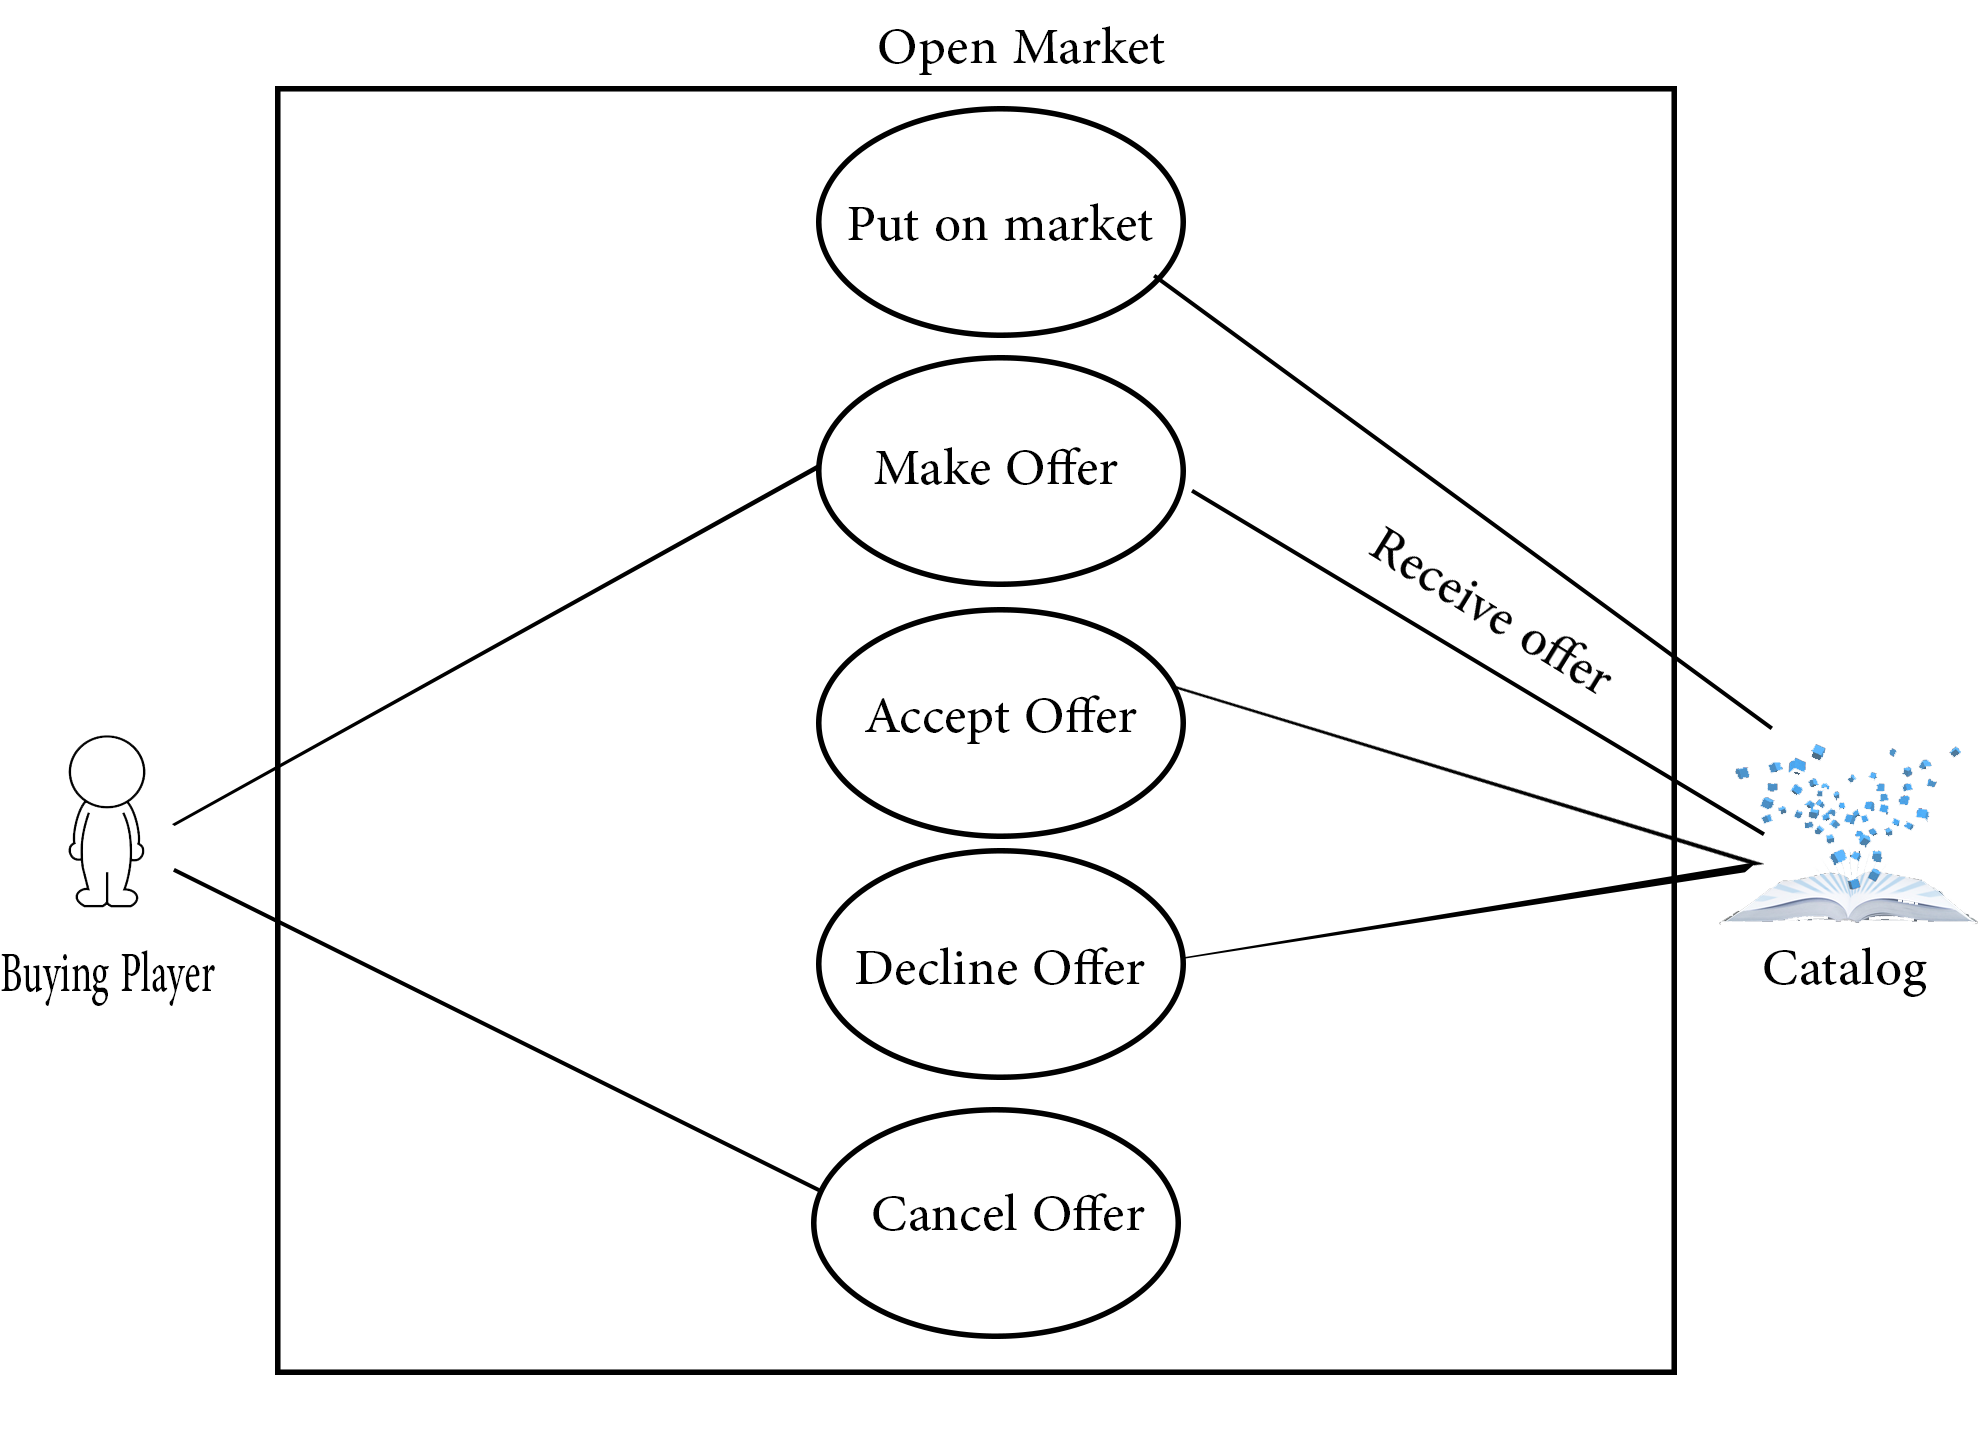
\includegraphics[width=550pt]{uml/useCaseDiagrams/buyUseCase.png}
    }
    \caption{Use Case Open Market}
\end{figure}
\subsubsection{Faire une offre}
\paragraph{Préconditions}
\begin{itemize}
 \item La partie est en cours.
 \item La propriété voulue n'appartient à personne.
\end{itemize}
\paragraph{Postconditions}
\begin{itemize}
 \item Une offre pour une propriété est envoyée.
\end{itemize}
\paragraph{Cas général}
A tout moment de la partie, n'importe quel joueur peut séléctionner une propriété dans le catalogue qui n'a pas de propriétaire, et faire une offre sur celle-ci. Après avoir séléctionner la propriété, ses informations sont affichées, et le joueur peut cliquer sur acheter.[Exception : Le joueur n'a pas assez d'argent]
\paragraph{Exceptions}
\begin{itemize}
 \item \textit{Le joueur n'a pas assez d'argent:} Une fenètre s'ouvre indiquant au joueur qu'il ne possède pas assez d'argent.
\end{itemize}

\subsubsection{Annuler une offre}
\paragraph{Préconditions}
\begin{itemize}
 \item La partie est en cours.
 \item Le joueur à fait une offre qui n'as pas encore été validée.
\end{itemize}
\paragraph{Postconditions}
\begin{itemize}
 \item L'offre est annulée et retirée.
\end{itemize}
\paragraph{Cas général}
Dès que le joueur a mit une offre et tant que celle-ci n'a pas été acceptée, ce joueur peut annuler cette offre.
\paragraph{Exceptions} Néant.

\subsubsection{Accepter une offre}
\paragraph{Préconditions}
\begin{itemize}
 \item La partie est en cours.
 \item Un joueur a fait une offre.
\end{itemize}
\paragraph{Postconditions}
\begin{itemize}
 \item Le joueur paie le prix de la propriété.
 \item Le joueur devient propriétaire de la propriété.
\end{itemize}
\paragraph{Cas général}
Lorsque le catalogue reçoit une offre sur un bâtiment, il accepte automatiquement celle-ci.[Exception : Deux joueur font la demande en même temps] Une fois l'offre acceptée, le joueur doit confirmer son achat ou l'annuler.
\paragraph{Exceptions}
\begin{itemize}
 \item \textit{Deux joueur font la demande en même temps:} La première offre reçue sera prise en compte, l'autre sera annulée.
\end{itemize}

\subsubsection{Mettre en vente}
\paragraph{Préconditions}
\begin{itemize}
 \item La partie est en cours.
 \item Il existe un bâtiment sans propriétaire.
\end{itemize}
\paragraph{Postconditions}
\begin{itemize}
 \item Le bâtiment est en vente libre.
\end{itemize}
\paragraph{Cas général}
Dès qu'un bâtiment n'as pas de prioritaire, le catalogue le met en vente libre. Les bâtiments créés en début de partie seront mit dans le catalogue, ainsi que les batiments d'un joueur qui vient de perdre qui sont mit en vente libre.
\paragraph{Exceptions} Néant.

\newpage
\subsection{Construire-Améliorer-Détruire}
\begin{figure}[ht]
    \makebox[\linewidth]{
        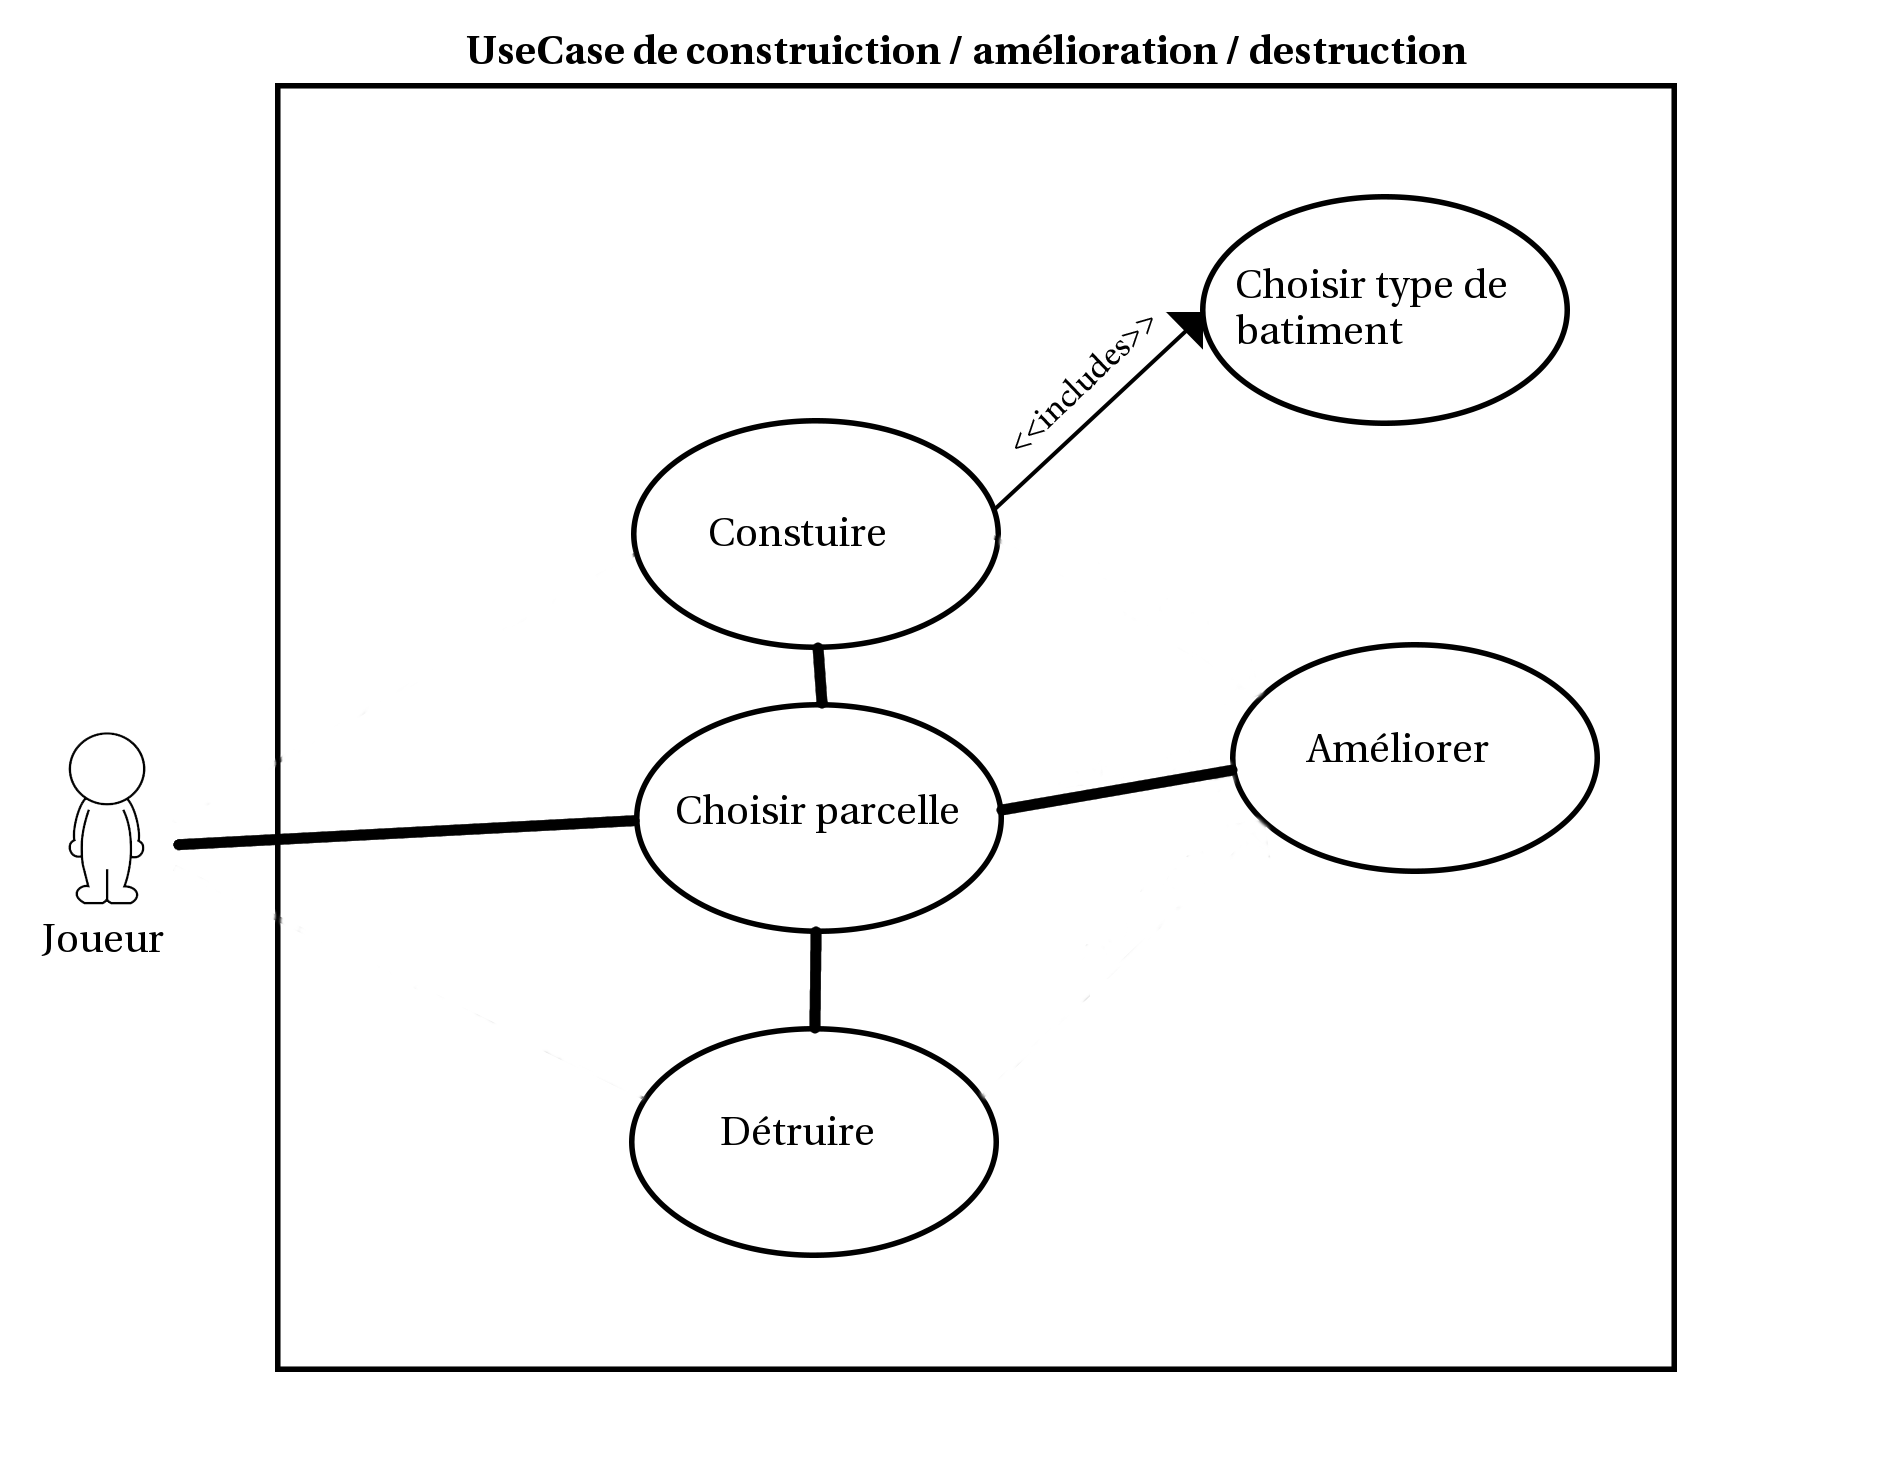
\includegraphics[width=550pt]{uml/useCaseDiagrams/buildDestroyUseCase.png}
    }
    \caption{Use Case Buid/Upgrade/Destroy}
\end{figure}
\subsubsection{Construire}
\paragraph{Obligations spéciales}
\begin{itemize}
 \item Inclut Select Building Map.
 \item Inclut Select Location.
\end{itemize}
\paragraph{Préconditions}
\begin{itemize}
 \item La partie est en cours.
 \item Le joeur possède au moins 1 parcelles vides.
\end{itemize}
\newpage
\paragraph{Postconditions}
\begin{itemize}
 \item Un bâtiment est construit.
 \item Le joueur possède ce nouveau bâtiment.
\end{itemize}
\paragraph{Cas général}
Lorsque un joueur veut construire un nouveau bâtiment, il lui faudra simplement séléctionner l'option \og \textit{Construire} \fg, il entre alors en mode Construction. Il peut à tout moment quitter ce mode et annuler la construction, en appuyant sur \og \textit{-ESC-} \fg ou en cliquant sur \og \textit{annuler} \fg. Un "catalogue" de type de bâtiment lui sera proposé, après qu'il en ai séléctionné un[Exception : Le joueur n'as pas assez d'argent], il devra cliquer sur le terrain sur lequel il veut construire.[Exception : Propriété séléctionnée non-valide]
\paragraph{Exceptions}
\begin{itemize}
 \item \textit{Le joueur n'as pas assez d'argent:}  Une fenètre s'ouvre indiquant au joueur qu'il ne possède pas assez d'argent.
 \item \textit{Propriété séléctionnée non-valide:}  Si le joueur séléctionne une proprité qui ne lui appartient pas, où qui ne possède déjà un bâtiment, une fenètre s'ouvre indiquant au joueur sa mauvaise sélection.
\end{itemize}
\subsubsection{Upgrade}
\paragraph{Obligations spéciales}
\begin{itemize}
 \item Inclut Select location.
\end{itemize}
\paragraph{Préconditions}
\begin{itemize}
 \item La partie est en cours.
\end{itemize}
\paragraph{Postconditions}
\begin{itemize}
 \item Un bâtiment est amélioré d'un niveau.
\end{itemize}
\paragraph{Cas général}
Un joueur peut à tout moment améliorer un de ses bâtiments. Il lui suffit de cliquer sur l'option \og \textit{Améliorer} \fg, il entre alors en mode Amélioration. Il peut à tout moment quitter ce mode et annuler l'amélioration, en appuyant sur \og \textit{-ESC-} \fg ou en cliquant sur \og \textit{annuler} \fg. Et ensuite séléctionner une de ses propriétés.[Exception : Bâtiment amélioré au max]Des informations sur l'amélioration sont affichés, le prix de celle-ci, et les stats du bâtiments après celle-ci.Il ne reste plus qu'au joueur de confirmer l'amélioration en cliquant sur \og \textit{Ok} \fg ou annuler en cliquant sur \og \textit{Annuler} \fg.[Exception : Le joueur n'as pas assez d'argent][Exception : Propriété séléctionnée non-valide]
\paragraph{Exceptions}
\begin{itemize}
 \item \textit{Le joueur n'as pas assez d'argent:}  Une fenètre s'ouvre indiquant au joueur qu'il ne possède pas assez d'argent.
 \item \textit{Propriété séléctionnée non-valide:}  Si le joueur séléctionne une proprité qui ne lui appartient pas, où qui ne possède pas de bâtiment, une fenètre s'ouvre indiquant au joueur sa mauvaise sélection.
 \item \textit{Bâtiment amélioré au max:}  Les bâtiments ont un niveau maximum d'amélioration Une fenètre s'ouvre indiquant au joueur qu'il ne peut plus améliorer ce bâtiment.
\end{itemize}
\subsubsection{Destroy}
\paragraph{Obligations spéciales}
\begin{itemize}
 \item Inclut Select location.
\end{itemize}
\paragraph{Préconditions}
\begin{itemize}
 \item La partie est en cours.
\end{itemize}
\paragraph{Postconditions}
\begin{itemize}
 \item Un bâtiment est détruit et n'éxiste plus.
\end{itemize}
\paragraph{Cas général}
Un joueur peut également détruire un de ses bâtiments. Il lui suffit de cliquer sur l'option \og \textit{Détruire} \fg, il entre alors en mode Destruction. Il peut à tout moment quitter ce mode et annuler la destruction, en appuyant sur \og \textit{-ESC-} \fg ou en cliquant sur \og \textit{annuler} \fg. Et ensuite séléctionner le bâtiment qu'il désire détruire.[Exception : Le joueur n'as pas assez d'argent] [Exception : Propriété séléctionnée non-valide]
\paragraph{Exceptions}
\begin{itemize}
 \item \textit{Le joueur n'as pas assez d'argent:}  Une fenètre s'ouvre indiquant au joueur qu'il ne possède pas assez d'argent.
  \item \textit{Propriété séléctionnée non-valide:}  Si le joueur séléctionne une proprité qui ne lui appartient pas, où qui ne possède pas de bâtiment, une fenètre s'ouvre indiquant au joueur sa mauvaise sélection.
\end{itemize}
\subsubsection{Select Building type}
\paragraph{Obligations spéciales}
\begin{itemize}
 \item Est inclut dans Build.
\end{itemize}
\paragraph{Préconditions}
\begin{itemize}
 \item Le joueur est entré en mode Construction.
\end{itemize}
\paragraph{Postconditions}
\begin{itemize}
 \item Un type est séléctionné pour la construction.
\end{itemize}
\paragraph{Cas général}
Un "catalogue" de types prédéfinis de bâtiment(bar,magasin,night-club,...) apparait, pour chaque type les statistiques (prix, coûts, capacité, heures,..) sont affichés. Il suffit au joueur alors de cliquer sur le type désiré.
\paragraph{Exceptions} Néant.

\newpage
\subsubsection{Select Location}
\paragraph{Obligations spéciales}
\begin{itemize}
 \item Est inclut dans Build.
 \item Est inclut dans Upgrade.
 \item Est inclut dans Destroy.
\end{itemize}
\paragraph{Préconditions}
\begin{itemize}
 \item Le joueur demande la construction/amélioration/destruction d'un bâtiment.
\end{itemize}
\paragraph{Postconditions}
\begin{itemize}
 \item Une propriété est séléctionnée pour la construction/amélioration/destruction et ses informations sont affichés.
\end{itemize}
\paragraph{Cas général}
Le joueur doit simplement cliquer, sur la carte, sur le terrain exigé.[Exception : Sélection invalide]
\paragraph{Exceptions}
\begin{itemize}
 \item \textit{Sélection invalide:} Si l'emplacement séléctionné n'est pas un terrain/bâtiment (et donc une route ou un obstacle), la sélection n'est pas faite.
\end{itemize}

\newpage
\subsection{Achats entre joueurs}
\begin{figure}[ht]
    \makebox[\linewidth]{
        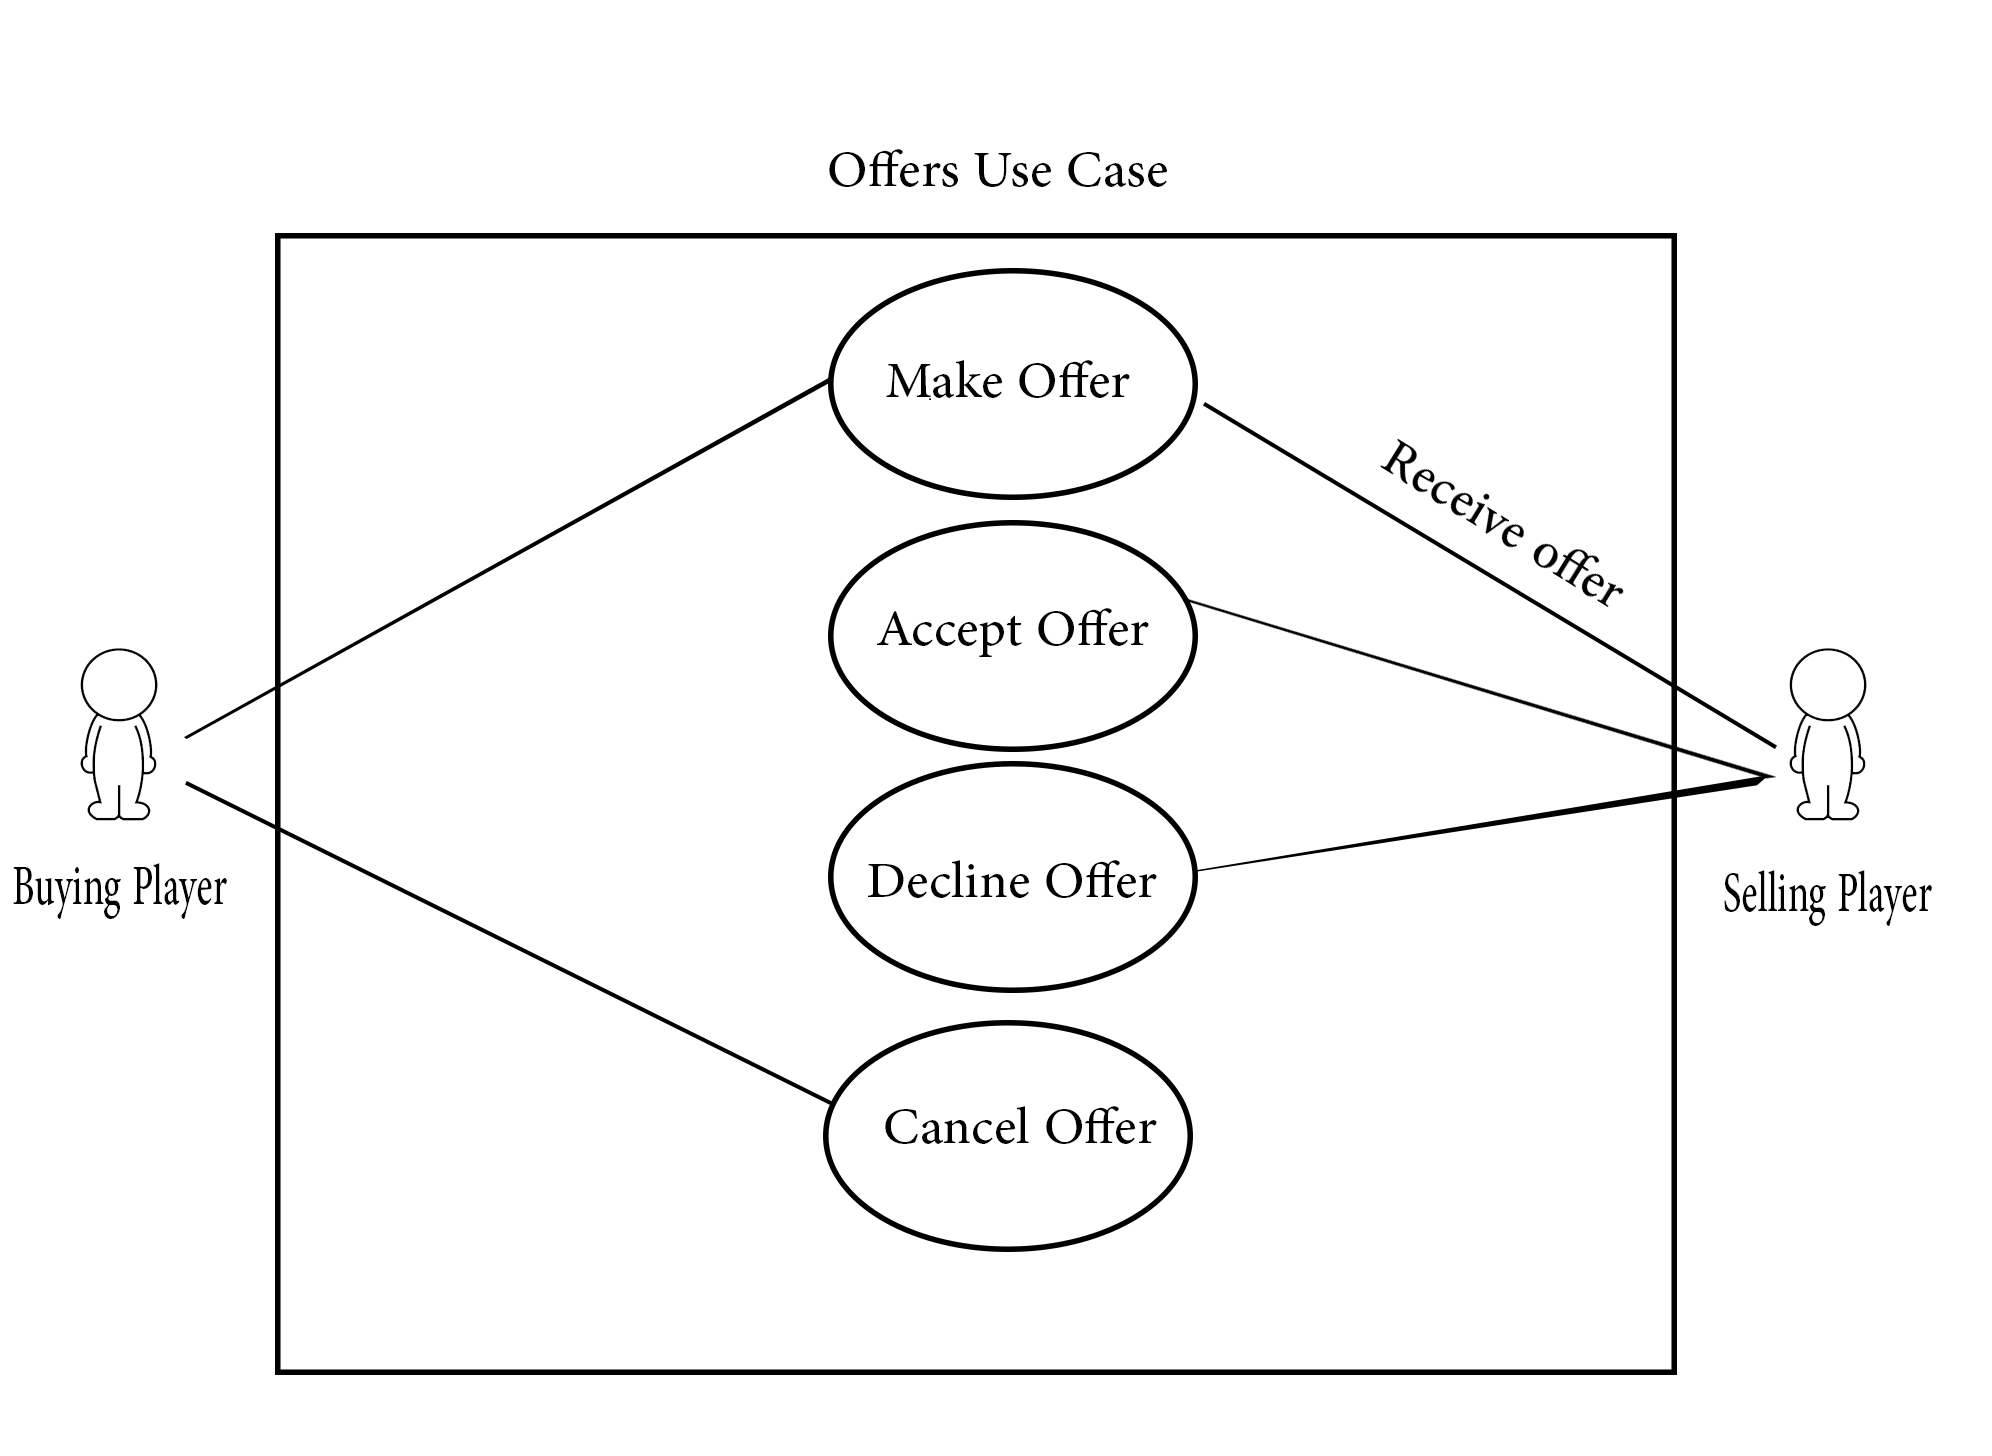
\includegraphics[width=550pt]{uml/useCaseDiagrams/offerUseCase.png}
    }
    \caption{Use Case between players sale}
\end{figure}
\subsubsection{Faire une offre}
\paragraph{Préconditions}
\begin{itemize}
 \item La partie est en cours.
 \item La propriété voulue appartient à un joueur.
\end{itemize}
\paragraph{Postconditions}
\begin{itemize}
 \item Une offre pour une propriété est envoyé à un autre joueur.
\end{itemize}
\paragraph{Cas général}
A tout moment de la partie, un joueur peut tenter d'acheter le bâtiment d'un autre. Il lui doit simplement de faire une offre auprès de ce joueur, pour ce bâtiment.[Exception : Le joueur a fait trop d'offre] Il suffit à l'acheteur de sélectionner le bâtiment voulu et de cliquer sur \og \textit{Faire une offre} \fg, une fenêtre s'ouvre pour que le joueur puisse donner le prix qu'il est prêt a payer et confirme son offre.[Exception : Le joueur n'a pas assez d'argent] 
\paragraph{Exceptions}
\begin{itemize}
 \item \textit{Le joueur n'a pas assez d'argent:} Une fenètre s'ouvre indiquant au joueur qu'il ne possède pas assez d'argent.
 \item \textit{Le joueur a fait trop d'offre:} Afin d'éviter tout spam, une limite d'offre sur un temps donné est instauré.
\end{itemize}
\subsubsection{Annuler une offre}
\paragraph{Préconditions}
\begin{itemize}
 \item La partie est en cours.
 \item Le joueur à fait une offre qui n'as pas encore été validée.
\end{itemize}
\paragraph{Postconditions}
\begin{itemize}
 \item L'offre est annulée.
\end{itemize}
\paragraph{Cas général}
Dès que le joueur a mit une offre et tant que celle-ci n'a pas été acceptée, ce joueur peut annuler cette offre.
\paragraph{Exceptions} Néant.
\subsubsection{Accepter une offre}
\paragraph{Préconditions}
\begin{itemize}
 \item La partie est en cours.
 \item Un joueur a reçu une offre.
\end{itemize}
\paragraph{Postconditions}
\begin{itemize}
 \item L'acheteur devient propriétaire de la propriété.
 \item Le vendeur reçoit une compensation monétaire et perd sa propriété.
\end{itemize}
\paragraph{Cas général}
Lorsque un joueur reçoit une offre sur un bâtiment, une fenêtre s'affiche avec les informations sur cette offre, il peut accepter celle-ci en cliquant sur \og \textit{Accepter} \fg.
\paragraph{Exceptions} Néant
\subsubsection{Refuser une offre}
\paragraph{Préconditions}
\begin{itemize}
 \item La partie est en cours.
 \item Un joueur a reçu une offre.
\end{itemize}
\paragraph{Postconditions}
\begin{itemize}
 \item L'offre est annulée.
\end{itemize}
\paragraph{Cas général}
Lorsque un joueur reçoit une offre sur un bâtiment, une fenêtre s'affiche avec les informations sur cette offre, il peut refuser celle-ci en cliquant sur \og \textit{Refuser} \fg.
\paragraph{Exceptions} Néant

\newpage
\section{Exigences non fonctionnelles}
\subsection{Service}
\paragraph{}
Le système fournira en premier lieu, l’assurance de la fonctionnalité du programme, et ce, sans bug ni ruptures.
\paragraph{}
Les différents outils du programme accompliront exactement la tâche décrite et demandée.
\paragraph{}
De plus, ces dites tâches seront claires et ne laisseront pas place à une ambiguïté quelconque.
Chaque outil du programme sera représenté par une image explicitant la fonction, et une explication claire sera accompagnée.
\paragraph{}
Le système sera esthétique et disposera donc d’une apparence conviviale, ludique, mais également professionnelle.
Celle-ci se distinguera par la qualité des textures utilisées, ainsi que par leur justesse par rapport aux informations qu’elles représentent.
\paragraph{}
Enfin, le système jouira d’une utilisabilité et d’une ergonomie agréable.
\subsection{Contraintes}
\paragraph{}
Afin de fonctionner correctement, et d’avoir une expérience de jeu optimale, le système devra être lancé sur un ordinateur possédant la configuration nécessaire.
En cas d’environnement peu performant, il est possible que des ralentissements, ou qu’un manque de fluidité se fasse ressentir.
\paragraph{}
Il est également nécessaire que le système soit accompagné d’une connexion internet stable et rapide.
Sans cela, la communication avec le serveur et entre les joueurs serait endommagée, et endommagerait la jouabilité de tous les joueurs.

\section{Exigences de domaine}
\begin{itemize}
 \item Le jeu est multijoueurs, et doit donc permettre aux différents utilisateurs de communiquer entre eux.
 \item Une partie doit être composé d'au minimum 2 joueurs et au maximum 8 joueurs.
 \item Les 8 premiers joueurs qui rejoingnent la partie seront les seules 8 joueurs capable de la rejoindre.
 \item Pour qu'un joueur puisse continuer à jouer, il doit posséder soit des terrains, des batiments ou encore avoir
 un capital. 
 \item Le capitale de chaque joueur varie tout au long de la partie en fonction des frais et des gains de chaque batiment.
 \item Les gains qu'apporte chaque batiment seront représentés par des visiteurs, qui, en suivant un chemin, pourront 
 rentrer dans un batiment qui augmentera le capital de son propiétaire.
 \item Si le joueur est en faillite, la partie se terminera pour ce joueur et il ne sera plus possible pour lui de
 continuer de jouer dans cette partie, mais il pourra toute fois la regarder.
 \item La partie se finie uniquement si il ne reste plus qu'un joueur propriétaire.

 \end{itemize}

\newpage
\chapter{Besoins du système}
\section{Exigences fonctionnelles}
\section{Exigences non fonctionnelles}
\section{Design et fonctionnement du système}
\begin{figure}[ht]
    \makebox[\linewidth]{
        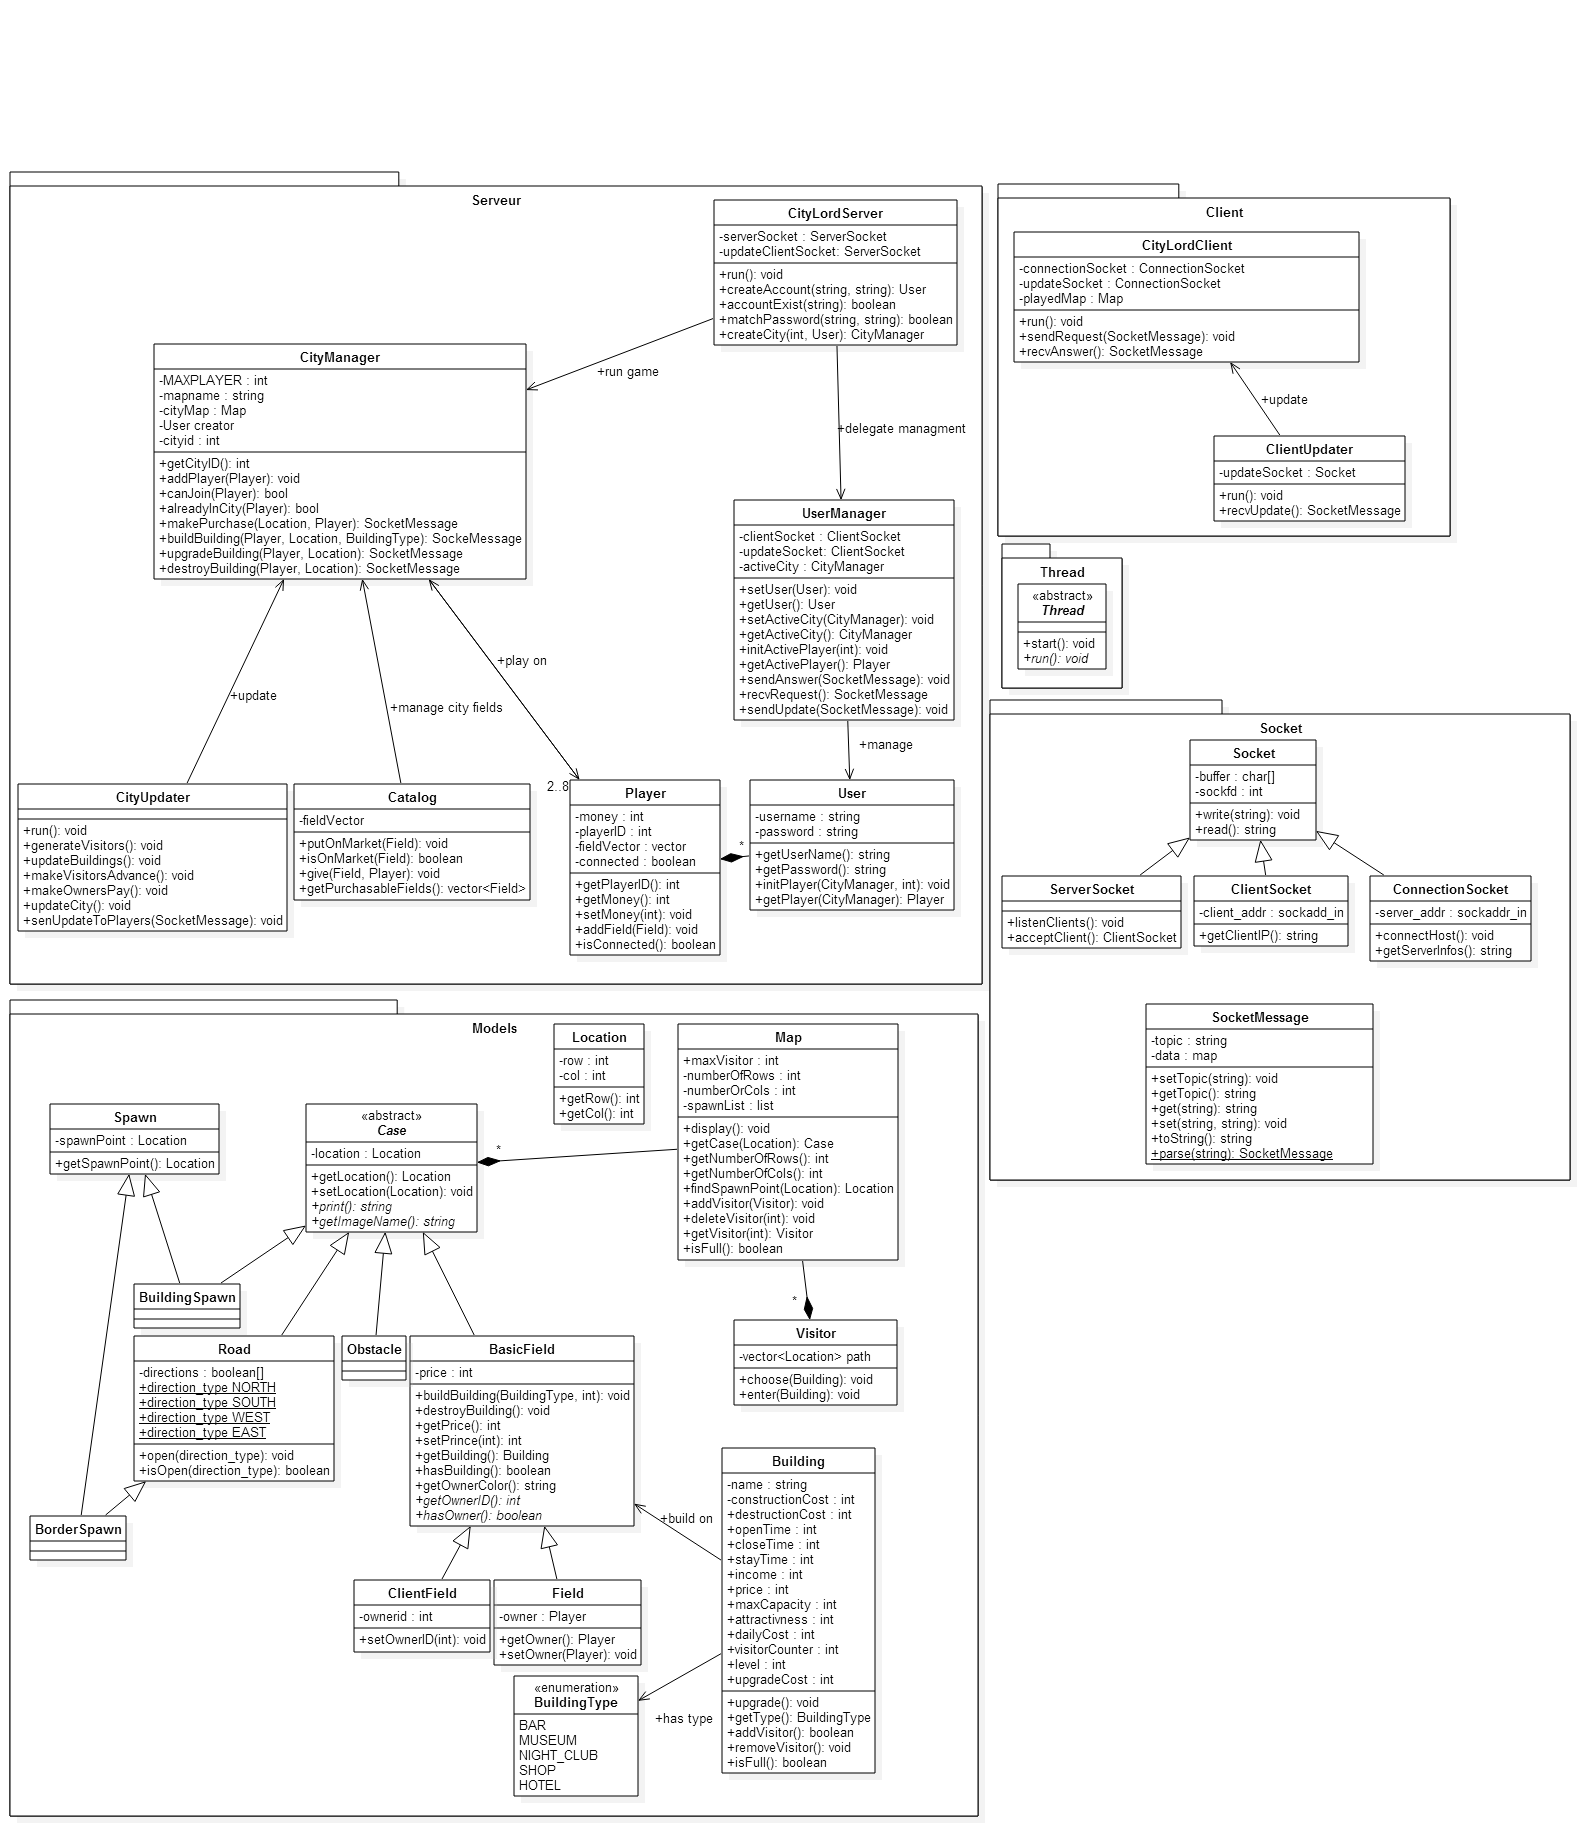
\includegraphics[width=550pt]{uml/classDiagrams/CD.png}
    }
    \caption{Diagramme de classe : Base du système}
\end{figure}


\newpage
\chapter{Index des termes utilisés}
\begin{itemize}
 \item \textbf{Catalogue}
 \item \textbf{Map}
 \item \textbf{Point-and-click}
 \item \textbf{Pseudo}
 \item \textbf{Réseau informatique}
 \item \textbf{Serveur}
 \item \textbf{Système}
\end{itemize}

\end{document}
